\section{\secfnwords}
\label{sec_fn_words}

Nearly all of the functions we have seen so far have had sets of numbers for their domain and codomain and have had rules defined by formulas.  In this section, we explore many new functions that have rules that are described in words, which include functions whose domain and codomain are sets of other discrete objects such as graphs and bit strings. 

%%%%%%%%%%%%%%%%%%%%%%%%%%%%%

\newcommand{\subfloorceiling}{Floor and Ceiling}
\subsection{\subfloorceiling}
\label{sub_floor_ceiling}

As a first example of functions with rules described in words, we consider the floor and ceiling functions which take a real (decimal) number input and find a nearby integer to output.  
 
\begin{defn}[Floor and ceiling]
\label{defn_floor_ceiling}
~
    \begin{apart}
        \item For a real number $x$, the \vocab{floor} of $x$, denoted $\lfloor x \rfloor$, is the result of rounding $x$ down to the nearest integer less than or equal to $x$. Officially, $\lfloor x \rfloor=k$ where $k$ is the greatest integer such that $k\le x$.  For example, $\lfloor 2.4 \rfloor = 2$ and $\lfloor -2.4 \rfloor = -3$. 
        This name comes from the fact that we look down to see the floor of a room. Notice that  the floor is the first integer at or to the left of the number on the real number line.

            \begin{figure}[htbp]
                \centering
                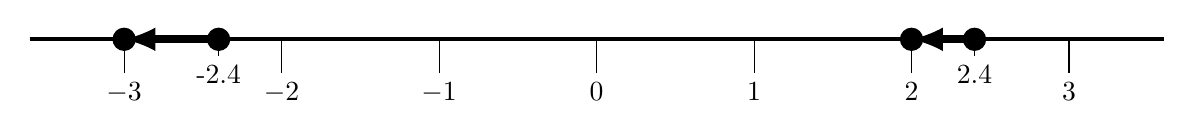
\begin{tikzpicture}[scale=2]
                %%%  Circles at points Note: white, thick OR white, very thick for open, black for closed.             
                \path [draw=black, fill=black] (2.4,0) circle (2.pt); 
                \path [draw=black, fill=black] (-2.4,0) circle (2.pt);         
                \path [draw=black, fill=black] (2,0.0) circle (2.pt); 
                \path [draw=black, fill=black] (-3,0.0) circle (2.pt); 
                %%% Vertical dash marks at points        
                \draw[shift={(2.4,0)},color=black] (0pt,0pt) -- (0pt,-3pt) node[below] {2.4}; 
                \draw[shift={(-2.4,0)},color=black] (0pt,0pt) -- (0pt,-3pt) node[below] {-2.4}; 
                \foreach \x in {-3,-2,-1,0,1,2,3}
                    \draw[shift={(\x,0)},color=black] (0pt,0pt) -- (0pt,-6pt) node[below] {$\x$}; 
                %%% Heavy arrows        
                \draw[draw=black,solid, -latex,line width=1mm,fill=black] (2.4,0) -- (2,0); 
                \draw[draw=black,solid, -latex,line width=1mm,fill=black] (-2.4,0) -- (-3,0); 
                %%% Axis with arrows
                %\draw[draw=black,solid, latex-latex,line width=0.5mm,fill=black] (-3.6,0) -- (3.6,0); 
                %%% Axis without arrows
                \draw[draw=black,solid,line width=0.5mm,fill=black] (-3.6,0) -- (3.6,0); 
                % Note:  layers from first command in order listed here.
                \end{tikzpicture}
                \caption{Calculating the floor by looking left on the real number line.}
                \label{fig_number_line_floor}
            \end{figure}

        \item For a real number $x$, the \vocab{ceiling} of $x$, denoted $\lceil x \rceil$, is the result of rounding $x$ up to the nearest integer greater than or equal to $x$.  Officially, $\lceil x \rceil =k$ where $k$ is the least integer such that $k\ge x$.  For example, $\lceil 2.4 \rceil = 3$ and $\lceil -2.4 \rceil = -2$.  This name comes from the fact that we look up to see the ceiling of a room. Notice that the ceiling is the first integer at or to the right of the number on the real number line.

            \begin{figure}[htbp]
                \centering
                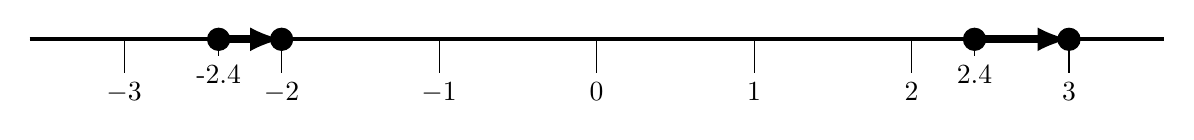
\begin{tikzpicture}[scale=2]
                %%%  Circles at points Note: white, thick OR white, very thick for open, black for closed.             
                \path [draw=black, fill=black] (2.4,0) circle (2.0pt); 
                \path [draw=black, fill=black] (-2.4,0) circle (2.0pt);         
                \path [draw=black, fill=black] (3,0.0) circle (2.0pt); 
                \path [draw=black, fill=black] (-2,0.0) circle (2.0pt); 
                %%% Vertical dash marks at points        
                \draw[shift={(2.4,0)},color=black] (0pt,0pt) -- (0pt,-3pt) node[below] {2.4}; 
                \draw[shift={(-2.4,0)},color=black] (0pt,0pt) -- (0pt,-3pt) node[below] {-2.4}; 
                \foreach \x in {-3,-2,-1,0,1,2,3}
                    \draw[shift={(\x,0)},color=black] (0pt,0pt) -- (0pt,-6pt) node[below] {$\x$}; 
                %%% Heavy arrows        
                \draw[draw=black,solid, -latex,line width=1mm,fill=black] (2.4,0) -- (3,0); 
                \draw[draw=black,solid, -latex,line width=1mm,fill=black] (-2.4,0) -- (-2,0); 
                %%% Axis with arrows
                %\draw[draw=black,solid, latex-latex,line width=0.5mm,fill=black] (-3.6,0) -- (3.6,0); 
                %%% Axis without arrows
                \draw[draw=black,solid,line width=0.5mm,fill=black] (-3.6,0) -- (3.6,0); 
                % Note:  layers from first command in order listed here.
                \end{tikzpicture}
                \caption{Calculating the ceiling by looking right on the real number line.}
                \label{fig_number_line_ceiling}
            \end{figure}
    \end{apart}
\end{defn}

Note that floor and ceiling are in the same level as parentheses in the order of operations (\Cref{defn_integer_algebra_order_operations}). Let's look at an example.

\begin{exam}[Floor and ceiling calculations]
\label{exam_floor_ceiling_calculate}
~
    \begin{apart}
        \item Evaluate $\lfloor \frac{10}{3} \rfloor$ and $\lfloor ^-\frac{10}{3} \rfloor$.
            \begin{soln}
                Since $\frac{10}{3} = 3.333\ldots$, we round down to get $\lfloor \frac{10}{3} \rfloor=3$.  Since $^-\frac{10}{3} = -3.333\ldots$, we round down (to a more negative number) to get -4. 
            \end{soln}        
        \item Evaluate $\lfloor 17 \rfloor$ and $\lceil 17 \rceil$.
            \begin{soln}
                Because 17 is an integer, we do not have to round at all. Therefore, $\lfloor 17 \rfloor = 17$ and $\lceil 17 \rceil = 17$.
            \end{soln}
    \end{apart}
\end{exam}

Try working with floor and ceiling. 

\begin{act}[Floor and ceiling]
\label{act_floor_ceiling} 
~
    \begin{actpart}
        \item Evaluate $\lfloor 1.4 \rfloor$ and $\lceil 1.4 \rceil$.
        \item Evaluate $\lfloor -15.82 \rfloor$ and $\lceil -15.82 \rceil$.
        \item Evaluate $\lfloor 308 \rfloor$ and $\lceil 308 \rceil$.
        \item Professor Dor\'ee expects 40 students to attend a talk. She wants to cans of sparkling water so each student can get one, then how many 12-packs of cans should she buy?  What if there are $n$ students? Your answer should involve $n$ and floor or ceiling.

    \item Give an example of a real number $x$ that is not an integer where $\lceil 2x \rceil = 2 \lceil x \rceil$.   Give a counterexample to the conjecture that $\lceil 2x \rceil = 2 \lceil x \rceil$ for all real numbers $x$. 
    
    \item Does there exist a real number $x$ where $\lfloor x \rfloor = 6$?  Is it unique?  How many real numbers $x$ have $\lfloor x \rfloor = 6$? Describe all real numbers $x$ such that $\lfloor x \rfloor = 6$.

    \item Consider a real number $x$ such that $\lfloor x \rfloor = 6$.  What is/are the possible value(s) of $\lceil x \rceil$?

    \item When is $\lfloor x \rfloor = \lceil x \rceil$ for a real number $x$? 

    \item If $x$ is a real number such that $\lfloor x \rfloor \neq \lceil x \rceil$, then how are $\lfloor x \rfloor$ and $\lceil x \rceil$ related?  State your answer in the form of a conjecture.  Be as specific as possible.

    \end{actpart}
\end{act}

We can define functions using floor and ceiling. 

\begin{exam}[Floor as a function]
\label{exam_floor_function}
    The function $\fn{floor}:\mathbb{R} \to \mathbb{Z}$ is defined by $\fn{floor}(x) = \lfloor x \rfloor$. 
        \begin{apart}
            \item Identify the domain and codomain of the function \fn{floor}.
                \begin{soln}
                    The domain of the function \fn{floor} is $\mathbb{R}$ and the codomain is $\mathbb{Z}$.
                \end{soln}
            \item Give an example of a real number $x$ such that $\fn{floor}(x) = 11$.  Now find a different real number $s$ such that $\fn{floor}(s)=11$.   
                \begin{soln}
                    Note that $\fn{floor}(11) = \lfloor 11 \rfloor = 11$ and so one example is $x=11$.  Another example is $x = 11.38$ because $\fn{floor}(11.38) = \lfloor 11.38 \rfloor = 11.$
                \end{soln}
            \item \label{part_floor11} Describe all real numbers $x$ such that $\fn{floor}(x)=11$. 
                \begin{soln}
                    Any real number $x$ that is 11 or larger, but not as larger as 12 will have $\fn{floor}(x)=11$.  We can describe these real numbers using the inequality $11 \le x < 12$ or the interval $[11,12)$.
                \end{soln}
        \end{apart}    
\end{exam}

%%%%%%%%%%%%%%%%%%%%%%%%%% 

\newcommand{\subnumberfn}{Number-theoretic Functions}
\subsection{\subnumberfn}
\label{sub_number_theoretic_functions}

Let's look at examples of functions with rules defined in words that come from number theory (\Cref{ch_number_theory}).  Here is a first example.

\begin{exam}[Number of divisors]
\label{exam_coundiv}
    The function $\fn{countdiv}: \mathbb{Z}^+ \to \mathbb{Z}^+$ is defined by
    $\fn{countdiv}(n)=$ the number of (positive) divisors of $n$.  
        \begin{apart}
            \item Evaluate $\fn{countdiv}(4)$.
                \begin{soln}
                    The divisors of four are: 1, 2, and 4.  Since there are three divisors, $\fn{countdiv}(4)=3$.
                \end{soln}
            \item Find an integer $n$ such that $\fn{countdiv}(n) = 4$.  Is it unique?  Explain.
                \begin{soln}
                    The integer six has four divisors: 1, 2, 3, and 6.  Therefore $\fn{coundiv}(6)=4$.  It is not unique because, for example, the integer ten also has four divisors: 1, 2, 5, and 10 and so $\fn{countdiv}(10)=4$ as well.
                \end{soln}
            \item Describe all integers with $\fn{countdiv}(n) = 4$.
                \begin{soln}
                    By our work in \Cref{sub_prime_fact}, there are two possible prime factorizations of a number having four positive divisors:  $p^3$ or $pq$ where $p$ and $q$ are distinct primes.  (If we made a divisor table, it would be $1 \times 4$ or $2 \times 2$.)
                \end{soln}
            \item Give a counterexample to the statement: for every positive integer $a$ and $b$, if $a<b$, then $\fn{countdiv}(a) < \fn{countdiv}(b)$.  It follows that the function $\fn{countdiv}$ is not increasing.
                \begin{soln}
                  We want an example that shows the statement is false, meaning it is a broken promise.  A counterexample is $a=6$ and $b=7$ because $6 < 7$ but $\fn{countdiv}(6)=4$ and $\fn{countdiv}(7) = 2$, so $\fn{countdiv}(6) \ge \fn{countdiv}(7)$.
                \end{soln}
        \end{apart}
\end{exam}

Practice with number-theoretic functions.

\begin{act}[Evaluating number-theoretic functions]
\label{act_number_functions} 
~    
    \begin{actpart}  
        \item The function $\fn{twopart}: \mathbb{N} \to \mathbb{N}$ defined by $\fn{twopart}(n)$ is the highest power of two that divides $n$. Note that $1 = 2^0$ is a power of two. Evaluate $\fn{twopart}(24)$, $\fn{twopart}(30)$, and $\fn{twopart}(31)$. 
        \item The function $\pi: \mathbb{N} \to \mathbb{N}$ defined by $\pi(n)=$ the number of primes less than or equal to $n$. Note that the function $\pi$ has nothing to do with the real number $\pi$. Evaluate $\pi(6)$ and $\pi(20)$.
        \end{actpart}
\end{act}

%%%%%%%%%%%%%%%%%%%%%%%%%%%%%%%%%%%%%%

\newcommand{\subfngraphs}{Graph-theoretic Functions}
\subsection{\subfngraphs}
\label{sub_graph_functions} 

Let's look at examples of functions with rules defined in words that come from graph theory (\Cref{ch_graph_theory}).  Here is a first example.

\begin{exam}[Count vertices of degree three]
\label{exam_count_vert_deg3}
    Let $\mathbb{G}_{10}$ denote the set of all graphs with ten vertices. The function $\fn{deg3}: \mathbb{G}_{10} \to \mathbb{N}$ is defined by $\fn{deg3}(G) =$ the number of vertices of $G$ that have degree 3. 
        \begin{apart}
            \item Identify the domain and codomain of $\fn{deg3}$.
                \begin{soln}
                    The domain is $\mathbb{G}_{10}$ and the codomain is $\mathbb{N}$. 
                \end{soln}
            \item Evaluate $\fn{deg3}(K_{3,7})$ where $K_{3,7}$ is the complete bipartite graph defined in \Cref{defn_complete_completebipartite}.
                \begin{soln}
                     The complete bipartite graph $K_{3,7}$ has three (black) vertices of degree seven and seven (white) vertices of degree three, so $\fn{deg3}(K_{3,7})=7$.
                \end{soln}
            \item Evaluate $\fn{deg3}(C_{10})$ where $C_{10}$ is the cycle defined in \Cref{defn_complete_completebipartite}.
                \begin{soln}
                     The cycle $C_{10}$ has ten vertices of degree two and, therefore, no vertices of degree three, so $\fn{deg3}(C_{10})=0$.
                \end{soln}
            \item Evaluate $\fn{deg3}(W_9)$ where $W_9$ is the wheel defined in \Cref{exam_wheel_ladder}.
                \begin{soln}
                     The wheel $W_9$ has one hub vertex of degree nine and nine outer vertices of degree three, so $\fn{deg3}(W_9)=9$.
                \end{soln}
            \item Evaluate $\fn{deg3}(L_{2 \times 5})$ where $L_{2 \times 5}$ is the ladder defined in \Cref{exam_wheel_ladder}.
                \begin{soln}                
                     The ladder $L_{2 \times 5}$ has four corner vertices of degree two and the other $10-4=6$ inner vertices have degree three, so $\fn{deg3}(L_{2 \times 5})=6$.  
                \end{soln}

            \item It turns out we can draw a graph $G$ with ten vertices such that $\fn{deg3}(G) = n$ for $n=0,1,2,3,4,5,6,7,8,9,$ and 10 and so the image of $\fn{deg3}$ is $\{0,1,2,3,4,5,6,7,8,9,10\}$.  Draw a graph $G$ with ten vertices such that $\fn{deg3}(G) = 2$. (Challenge yourself to draw the others.)
                \begin{soln}
                    One such graph is drawn in \Cref{fig_two_deg3}.
                        \begin{figure}[hb]
                            \centering
                            %Used in \Cref{sec_functions}.

\begin{tikzpicture}
    [scale =.5]
    \GraphInit[vstyle=Welsh]
    \SetGraphUnit{2}
        \SetVertexNoLabel
    % bottom row
    \Vertex[LabelOut,Lpos=90,x=0,y=0]{a1}
    \Vertex[LabelOut,Lpos=90,x=1.5,y=0]{b1} 
    \Vertex[LabelOut,Lpos=90,x=3,y=0]{c1}
    \Vertex[LabelOut,Lpos=90,x=4.5,y=0]{d1}    
    \Vertex[LabelOut,Lpos=90,x=6,y=0]{e1}
    \Edges(a1,b1,c1,d1,e1)
    % middle row
    \Vertex[LabelOut,Lpos=90,x=0,y=1.5]{a2}
    \Vertex[LabelOut,Lpos=90,x=1.5,y=1.5]{b2} 
    \Vertex[LabelOut,Lpos=90,x=3,y=1.5]{c2}
    \Vertex[LabelOut,Lpos=90,x=4.5,y=1.5]{d2}   
    \Vertex[LabelOut,Lpos=90,x=6,y=1.5]{e2}
    \Edges(a2,b2,c2,d2,e2)
    % vertical edges
    \Edges(a1,a2)
    \Edges(c1,c2)
    \Edges(e1,e2)
\end{tikzpicture}
                            \caption{A graph with exactly two vertices of degree three from \Cref{exam_count_vert_deg3}.}
                            \label{fig_two_deg3}
                        \end{figure}
                \end{soln}
         \end{apart}
\end{exam}

Try working with functions that involve graphs.

\begin{act}[Graph-theoretic functions]
\label{act_graph_theoretic_functions}
    Throughout this activity, $\mathbb{G}$ denotes the set of all graphs.
        \begin{actpart}
            \item The function $\fn{comp}: \mathbb{G} \to \mathbb{G}$ is defined by $\fn{comp}(G)=\overline{G}$, the graph theoretic complement of the graph $G$. Evaluate (draw) $\fn{comp}(W_4)$ for the wheel graph $W_4$.
            \item The function $c: \mathbb{G} \to \mathbb{N}$ is defined by $c(G)=$ the the number of edges in of the longest path in $G$. Evaluate $c(C_5)$ for the cycle $C_5$ and $c(K_{1,4})$ for the complete bipartite graph (star) $K_{1,4}$.
            \item The function $\fn{isplanar}: \mathbb{G} \to \{0,1\}$ is defined by 
                $$\fn{isplanar}(G) 
                = \left\{ \begin{array} {cl} 
                0 & \text{if }G\text{ is planar} \\
                1 & \text{if }G\text{ is not planar} \\
                \end{array} \right.$$
            \item Evaluate $\fn{isplanar}(C_5)$ and $\fn{isplanar}{K_5}$ for the cycle $C_5$ and the complete graph $K_5$.  Hint: $K_5$ is not planar.
        \end{actpart}
\end{act}

%%%%%%%%%%%%%%%%%%%%%%%%%%%%%%%%%%%%%%
\newcommand{\subbitstringfunctions}{Functions Involving Bit Strings}
\subsection{\subbitstringfunctions}
\label{sub_bit_string_functions}

Next, let's look at functions defined on bit strings. We defined bit strings, the length of a bit string, and the weight of a bit string in \Cref{defn_bit_string}.  We start by establishing the notation for the empty string and for sets of bit strings.

\begin{defn}[Sets of bit strings]
\label{defn_sets_bit_strings}
~
    \begin{apart}
        \item The symbol\footnote{The lowercase Greek letter lambda, denoted $\lambda$, is similar to the English letter \str{l}.} $\lambda$ represents the \vocab{empty bit string}.  It has length and weight 0. 
        
        \item The \vocab{set of all bit strings} is the set $$\mathbb{B} = \{ \lambda, \bs{0}, \bs{1}, \bs{00}, \bs{01}, \bs{10}, \bs{11}, \bs{000}, \bs{001}, \bs{010}, \bs{011}, \bs{100}, \bs{101}, \bs{110}, \bs{111}, \bs{0000}, \bs{0001}, \bs{0010}, \bs{0011}, \ldots \}.$$

        \item The \vocab{set of all non-empty bit strings} is the set $\mathbb{B}$ without $\lambda$, namely
        $$\mathbb{B}^* = \{\bs{0}, \bs{1}, \bs{00}, \bs{01}, \bs{10}, \bs{11}, \bs{000}, \bs{001}, \bs{010}, \bs{011}, \bs{100}, \bs{101}, \bs{110}, \bs{111}, \bs{0000}, \bs{0001}, \bs{0010}, \bs{0011}, \ldots \}.$$

        \item For any non-negative integer $n$, the set of all bit strings of length $n$ is $\mathbb{B}_n.$
        For example, $\mathbb{B}_0 = \{\lambda\}$, $\mathbb{B}_1 = \{\bs{0}, \bs{1}\}$, $\mathbb{B}_2 = \{\bs{00}, \bs{01}, \bs{10}, \bs{11}\}$ and 
        $$\mathbb{B}_3 = \{\bs{000}, \bs{001}, \bs{010}, \bs{011},\bs{100}, \bs{101}, \bs{110}, \bs{111}\}.$$
    \end{apart}
\end{defn}

Let's look at an example of a function on bit strings.

\begin{exam}[Weight function on bit strings]
\label{exam_weight_function_bit_strings}
    Consider the function $\fn{wgt}: \mathbb{B} \to \mathbb{Z}$ defined by $\fn{wgt}(b) =$ weight of the bit string $b$.
        \begin{apart}
            \item What are the domain and codomain of the function $\fn{wgt}$?
                \begin{soln}
                    The domain is the set of all bit strings, $\mathbb{B}$, and the codomain is the set of all integers, $\mathbb{Z}$.
                \end{soln}
            \item Evaluate $\fn{wgt}(\bs{001})$, $\fn{wgt}(\bs{1111})$, and $\fn{wgt}(\lambda)$.
                \begin{soln}
                    The weight of a bit string is the number of \bs{1}s in the bit string.  Since \bs{001} has one \bs{1}, $\fn{wgt}(\bs{001})=1$.  Since \bs{1111} has four \bs{1}s, $\fn{wgt}(\bs{1111})=4$.  Since $\lambda$ has no \bs{1}s, $\fn{wgt}(\lambda)=0$.
                \end{soln}
            
            \item \label{part_weight0}
            Describe all bit strings $b$ such that $\fn{wgt}(b)=0$.
                \begin{soln}
                    For a bit string to have weight 0, it cannot contain any \bs{1}s. That is, it must be empty or entirely \bs{0}s. We can list such strings as $\lambda, \bs{0}, \bs{00}, \bs{000},  \bs{0000}, \ldots.$
                \end{soln}
            \item \label{part_weightn} 
            For a positive integer $n$, describe a bit string $b$ such that $\fn{wgt}(b) = n$.
                \begin{soln}
                    We are looking for a bit string $b$ that has weight $n$ or, equivalently, that contains $n$ \bs{1}s.  The simplest example is $$b = \underbrace{\bs{11}\ldots\bs{1}}_{n},$$
                    the bit string with $n$ 1s.  Other answers are possible, such as $$b = \bs{0}\underbrace{\bs{11}\ldots\bs{1}}_{n }\bs{0},$$ 
                \end{soln}
            \item What is the image of the function $\fn{wgt}$?
                \begin{soln}
                    It is not possible to have a negative weight.  We saw in (\ref{part_weightn}) and (\ref{part_weight0}) that any non-negative integer is the weight of some bit strings.  Therefore, the image of \fn{wgt} is $\mathbb{N}$.
                \end{soln}
        \end{apart}   
\end{exam}

It is your turn to practice with functions on bit strings.

\begin{act}[Functions on bit strings]
\label{act_functions_bit_strings}
~
        \begin{apart}   
            \item The function $l:\mathbb{B} \to \mathbb{Z}$ defined by $l(b) =$ the length of the bit string $b$. Evaluate $l(\bs{0})$ and $l(\bs{1011})$.
            
            \item The function $\fn{lastbit}:\mathbb{B}^* \to \mathbb{B}$ defined by $\fn{lastbit}(b) =$ the last bit in the bit string $b$. Evaluate $\fn{lastbit}(\bs{0})$ and $\fn{lastbit}(\bs{1011})$.
            
            \item The function $\fn{append}: \mathbb{B}\to \mathbb{B}^*$ defined by $\fn{append}(b)=b\bs{1}$, literally the string $b$ with a \bs{1} added to the right. Evaluate $\fn{append}(\bs{0})$ and $\fn{append}(\bs{1011})$.

            \item The function $\fn{reverse}:\mathbb{B}\to \mathbb{B}$ defined by $\fn{reverse}(b)=\overleftarrow{b}$, where $\overleftarrow{b}$ means the bit string $b$ written in reverse order. Evaluate $\fn{reverse}(\bs{0})$ and $\fn{reverse}(\bs{1011})$.

            \item The function $f:\mathbb{B}^*\to \mathbb{B}$ defined by $$f(b)= \left\{ \begin{array} {ll} b & \text{if the last bit of the bit string } b \text{ is } \bs{0} \\ b \text{ without its last  bit}  & \text{if the last bit of the bit string } b \text{ is } \bs{1} \\  \end{array} \right.$$ Evaluate $f(\bs{0})$ and $f(\bs{1011})$.

            \item Define a simple-to-describe function $g:\mathbb{B}^*\to \mathbb{B}^*$ such that $g(\bs{1011}) = \bs{0100}$, $g(\bs{110})= \bs{001}$, and $g(\bs{000011}) = \bs{111100}$. % Answer: twos complement

            \item Define a simple-to-describe function $h:\mathbb{B}^*\to \mathbb{B}^*$ such that $g(\bs{1011}) = \bs{10111}$, $g(\bs{110})= \bs{1100}$, and $g(\bs{000011}) = \bs{0000110}$.  Hint: even. % Answer append last bit to get even weight
        \end{apart}
\end{act}

%%%%%%%%%%%%%%%%%%%%%%%%%%%%%%%%%%%%%%%%%%%

\subsection{Exercises}

%%%%%%%%%%%%%%%%%%%%%%%%

\subsubsection*{Exercises for \Cref{sub_floor_ceiling} \subfloorceiling}

\begin{exer}[\exerP] % calculate floor and ceiling]
\label{exer_floor_ceiling_calculate}
    In this exercise, evaluate without using technology.
        \begin{exerpart}
            \item Evaluate $\lfloor 14.5 \rfloor$, $\lfloor 14 \rfloor$, and $\lfloor -14.5 \rfloor$.
            \item Evaluate $\lceil 14.5 \rceil$, $\lceil 14 \rceil$, and $\lceil -14.5 \rceil$.
            \item Evaluate $\left\lfloor \frac{7}{3} \right\rfloor$ and $\left\lceil \frac{7}{3} \right\rceil$.
        \end{exerpart}
\end{exer}

\begin{exer}[\exerP] % order ops with floor and ceiling
\label{exer_floor_ceiling_order_ops}
    In this exercise, evaluate without using technology.
        \begin{exerpart}
            \item Evaluate $\lfloor 0.7 + 0.5 \rfloor$.
            \item Evaluate $\lceil 9.5 \rceil  -  \lfloor 9.5 \rfloor$.
            \item Evaluate $\lfloor \lceil 103.4 \rceil \rfloor$. 
        \end{exerpart}
\end{exer}

\begin{exer}[\exerP] % the ceiling function]
\label{exer_ceiling_function}
    The function $\fn{ceil}: \mathbb{R} \to \mathbb{Z}$ is defined by $\fn{ceil}(x) = \lceil x \rceil$.   
        \begin{exerpart}
            \item Identify the domain and codomain of the function \fn{ceil}.
            \item Evaluate $\fn{ceil}(60.7)$, $\fn{ceil}(60)$, and $\fn{ceil}(61)$.
            \item Give an example of a real number $x$ such that $\fn{ceil}(x) = 11$.  Now find a different real number $s$ such that $\fn{ceil}(x)=11$.
            \item Describe all real numbers $x$ such that $\fn{ceil}(x)=11$. Answer using an inequality and also using interval notation.
        \end{exerpart}
\end{exer}

\begin{exer}[\exerU] % Floor counterexamples
\label{exer_floor_cex}
    Each of the following statements is false. Find a counterexample.
        \begin{exerpart}
            \item For any real number $x$, we have $10 \lceil x \rceil = \lceil 10x \rceil .$
            \item  For any real numbers $x$ and $y$, if $x > y$, then $\lfloor x \rfloor > \lfloor y \rfloor$.  
        \end{exerpart}
\end{exer}

\begin{exer}[\exerU] % floor of sum and ceiling of product]
\label{exer_floor_sum_ceiling_product}   
~
    \begin{exerpart}
        \item Give an example of real numbers $x$ and $y$ that are not integers such that $\lfloor x +y \rfloor = \lfloor x \rfloor + \lfloor y \rfloor.$

        \item Give a counterexample to the conjecture that $\lfloor x +y \rfloor = \lfloor x \rfloor + \lfloor y \rfloor$ for all real numbers $x$ and $y$.

        \item Give an example of real numbers $x$ and $y$ that are not integers such that $\lceil xy \rceil = \lceil x \rceil \lceil y \rceil.$

         \item Give a counterexample to the conjecture that $\lceil xy \rceil = \lceil x \rceil \lceil y \rceil$ for all real numbers $x$ and $y$.
    \end{exerpart}
\end{exer}

\begin{exer}[\exerU] % floor of negative]
\label{exer_floor_negative}
~
    \begin{exerpart}
        \item Give an example of a real number $x$ where $$\lfloor -x \rfloor \neq -\lfloor x \rfloor.$$
        \item Make a conjecture about how $\lfloor -x \rfloor$ can be simplified to an expression with the negative sign on the outside. 
    \end{exerpart}
\end{exer}

\begin{exer}[\exerU] % floor of $\frac{n-1}{3}$]
\label{exer_floor_nover3}
    The function $h: \mathbb{N} \to \mathbb{N}$ is defined by $h(n) = \left\lfloor \frac{n+1}{3} \right\rfloor$. 
        \begin{exerpart}
        \item Explain why $\left\lfloor \frac{n+1}{3} \right\rfloor$ is always a nonnegative integer.
        \item Identify the domain and codomain of the function $h$.
        \item Evaluate $h(4)$, $h(5)$, and $h(6)$.
        \item Draw the dot diagram for $h$ showing at least $n=0,1,2,3,4,5,6$.  
        \end{exerpart}
\end{exer}

\begin{exer}[\exerR] % floor and ceiling
\label{exer_dyk_floor_ceil}
    Do you know \ldots
        \begin{exerpart}
            \item What the symbols $\lfloor ~ \rfloor$ and $\lceil ~ \rceil$ mean?
            \item How to build counterexamples involving floor and ceiling?
            \item When to use floor versus ceiling in an applied problem?
        \end{exerpart}
\end{exer}

\begin{exer}[\exerE] % formulas for \fn{div} and \fn{mod}]
\label{exer_div_mod_formulas} 
~
    \begin{exerpart}
        \item Calculate $20 \fn{ div } 7$ and $20 \fn{ mod } 7$ by hand.
        \item \label{part_formula_div} Write a formula for $a \fn{ div } n$ in terms of $a$ and $n$.  Use $\frac{a}{n}$, not $a \div n$, in your formula.  Hint: Your answer should involve floor or ceiling.
        \item Use your answer to (\ref{part_formula_div}) to write a formula for $a \fn{ mod } n$ in terms of $a$ and $n$.
        \end{exerpart}
\end{exer}

\begin{exer}[\exerE] % $x \mapsto \lfloor x + 0.5\rfloor$]
\label{exer_rounding_off_function}
    The function $r: \mathbb{R} \to \mathbb{R}$ is defined by $r(x)= \lfloor x + 0.5\rfloor$.
        \begin{exerpart}
            \item Evaluate $r(2)$, $r(2.4)$, $r(2.6)$, and $r(2.5)$.
            \item Evaluate $r(-1)$, $r(-1.3)$, $r(-1.7)$, and $r(-2.5)$.
            \item Describe the effect of the function $r$ in words.
        \end{exerpart}   
\end{exer}

%%%%%%%%%%%%%%%%%%%%%%%%%%%%%%

\subsubsection*{Exercises for \Cref{sub_number_theoretic_functions} \subnumberfn}

\begin{exer}[\exerP] % reading new definitions of number-theoretic functions
\label{exer_number_fn_readnew}
~
    \begin{exerpart}
        \item The function $g: \mathbb{N} \to \mathbb{N}$ is defined by $g(n)=$ the largest integer less than or equal to $\sqrt{n}$. Evaluate $g(17)$, $g(30)$, and $g(9)$. Show work.
        \item The function $\fn{fivepart}: \mathbb{N} \to \mathbb{N}$ is defined by $\fn{fivepart}(n)$ is the highest power of five that divides $n$. Note that $1 = 5^0$ is a power of five. Evaluate $\fn{fivepart}(30)$, $\fn{fivepart}(24)$, and $\fn{fivepart}(75)$. Show work
        \item  The function $f:\mathbb{Z}^+ \to \mathbb{Z}^+$ defined by $f(n)=$ the number of distinct positive primes that divide $n$. Evaluate $f(12)$, $f(16)$, $f(30)$, and $f(1)$. Show work.
    \end{exerpart}
\end{exer}

\begin{exer}[\exerP] % multiple of 2 or 5
\label{exer_fn_mult2_mult5}  
    Consider the function $t: \mathbb{Z}^+ \to \mathbb{Z}$ defined by 
        $$t(n)= \left\{ \begin{array} {cl}
            2 & \text{if } 2 \mid n \land 5 \mid n \\
            1 & \text{if } 2 \mid n \oplus 5 \mid n \\
            0 & \text{if } 2 \nmid n \land 5 \nmid n
        \end{array} \right.$$
    Recall $\land$ means ``and'' whereas $\oplus$ means ``xor'', the exclusive or.
        \begin{exerpart}
            \item Evaluate $t(20)$ and $t(6)$.  Show work.
            \item Describe the image of $t$.
            \item How many integers $n$ between 1 and 20 have $t(n) = 0$?  List them.
        \end{exerpart}
\end{exer}

\begin{exer}[\exerP] %Top prime
\label{exer_eval_topprime}
    Consider the function $\fn{gplt}:\mathbb{Z}^+ \to \mathbb{N}$ defined by     
            $$\fn{gplt}(n)=\left\{\begin{array}{cl}
                    0 & \text{if }n=1 \\
                    \text{the largest prime less than or equal to }n & \text{if } n \ge 2 \\
            \end{array}\right.$$
    The \fn{gplt} stands for ``greatest prime less than''.
    \begin{exerpart}
        \item Evaluate $\fn{gplt}(16)$.  Show work.
        \item Make a table showing the values of $\fn{gplt}(n)$ for $n=1,2,3,\ldots 20$.
        \item Draw the dot diagram for the function $\fn{gplt}$ showing $\fn{gplt}(n)$ for $n=1,2,3,\ldots 20$.
    \end{exerpart}
\end{exer}

\begin{exer}[\exerU] % counting divisors function]
\label{exer_countdiv}
    In \Cref{exam_coundiv}, we defined the function $\fn{countdiv}: \mathbb{Z}^+ \to \mathbb{Z}^+$ is defined by $\fn{countdiv}(n)=$ the number of (positive) divisors of $n$.
        \begin{exerpart}
            \item Make a table showing the values of $\fn{countdiv}(n)$ for $n = 1, 2, 3, 4, 5, 6, 7, 8, 9, 10$.
            \item What's the name for a number $n$ with $\fn{countdiv}(n) = 2$?
            \item Find a value of $n$ such that $\fn{countdiv}(n) = 5$.  Now find another.
            \item What can you say about $n$ if $\fn{countdiv}(n)$ is odd?  Hint: Lockers Puzzle (\Cref{act_lockers}). 
        \end{exerpart}
\end{exer}

\begin{exer}[\exerU] %Euler's phi function revisited
\label{exer_fn_euler_phi_revisited}
    Recall from \Cref{defn_euler_phi_fn} that Euler's phi function $\phi: \mathbb{Z}^+ \to \mathbb{Z}^+$ is defined by $\phi(n)=$ the number of integers between 1 and $n$ that are coprime to $n$.  
        \begin{exerpart}
            \item Identify the domain and codomain of $\phi$.
            \item Evaluate $\phi(12)$.  Show work.
            \item Describe all integers $n$ such that $\phi(n)=n-1$.
            \item Give a counterexample to the conjecture: for all positive integers $a$ and $b$, if $a < b$, then $\phi(a) < \phi(b)$.
        \end{exerpart}
\end{exer}

% SU:  you should have an exercise about the function lg defined!!

\begin{exer}[\exerU] % odd numbers less than or equal to]
\label{exer_odd_numbers_less_than}
    The function $\fn{oddless}:\mathbb{N} \to \mathbb{N}$ is defined by $\fn{oddless}(n) =$ the number of positive odd integers less than or equal to $n$.
        \begin{exerpart}
            \item List the positive odd integers less than or equal to five.  
            \item Evaluate $\fn{oddless}(5)$ and $\fn{oddless}(6)$.
            \item Draw the dot diagram for the function $\fn{oddless}$ showing $\fn{oddless}(n)$ for $n=0,1,2,3,4,5,6$.
            \item Write a formula for the rule for $\fn{oddless}$. Hint: The floor or ceiling is involved.
        \end{exerpart}
\end{exer}

\begin{exer}[\exerR] % number-theoretic functions
\label{exer_dyk_number_functions}
    Do you know \ldots
        \begin{exerpart}
            \item How to read definitions of functions involving divisors, primes, and other number-theoretic quantities?
            \item How $\fn{countdiv}(n)$, $\pi(n)$, and $\phi(n)$ are defined? (These are famous functions.)
        \end{exerpart}
\end{exer}

\begin{exer}[\exerE]
\label{exer_prime_counting_function}
    Read more about the function the prime counting function $\pi$ defined in \Cref{act_number_functions}.  For example, see Wikipedia \url{https://en.wikipedia.org/wiki/Prime-counting_function} What does the prime number theorem say?
\end{exer}

\begin{exer}[\exerE] % function involving ceiling and log]
\label{exer_number_digits_revisited}
     The function $g: \mathbb{Z}^+ \to \mathbb{Z}$ is defined by $g(n) = \lfloor \fn{log}(n) \rfloor + 1$.
         \begin{exerpart}
             \item Evaluate $g(1000)$ without using a calculator.
             \item Evaluate $g(6)$, $g(67)$, $g(678)$, and $g(6789)$.  Use technology (calculator or Internet search) to evaluate the necessary logs.
             \item Describe what $g$ is counting.  
         \end{exerpart}
\end{exer}

%%%%%%%%%%%%%%%%%%%%%%%%%%%%%%%%%%%%%
\subsubsection*{Exercises for \Cref{sub_graph_functions} \subfngraphs}

\begin{exer}[\exerP] % Counting leaves function
\label{exer_count_leaf_function}
    Let $\mathbb{G}_{10}$ denote the set of all graphs with ten vertices.  The function $\fn{cleaf}: \mathbb{G}_{10} \to \mathbb{N}$ is defined by $\fn{cleaf}(G)$ is the number of leaves (degree 1 vertices) in the graph $G$.
        \begin{exerpart}
            \item Evaluate $\fn{cleaf}(P_{10})$, $\fn{cleaf}(K_{1,9})$, and $\fn{cleaf}(C_{10})$ for the path $P_{10}$, the complete bipartite graph (star) $K_{1,9}$, and the cycle $C_{10}$.
            \item Draw a graph $G$ with ten vertices and $\fn{cleaf}(G)=0$.
            \item Draw a graph $G$ with ten vertices and $\fn{cleaf}(G)=5$.
        \end{exerpart}         
\end{exer}

\begin{exer}[\exerP] % chromatic number function on graphs
\label{exer_chromatic_number_function}
    Let $\mathbb{G}_{10}$ denote the set of all graphs with ten vertices. The function $\chi: \mathbb{G}_{10} \to \mathbb{N}$ is defined by $\chi(G)$ is the chromatic number of the graph $G$, as defined in \Cref{defn_chromatic_number}. 
        \begin{exerpart}
            \item Identify the domain and codomain of $\chi$.
            \item Evaluate $\chi(C_{10})$ and $\chi(K_{10})$ for the cycle $C_{10}$ and the complete graph $K_{10}$.
            \item Draw graph $G$ with ten vertices and $\chi(G)=3$. 
        \end{exerpart}   
\end{exer}

\begin{exer}[\exerP] %longest path function
\label{exer_longest_path_fn}
    Let $\mathbb{G}$ denote the set of all graphs. The function $c: \mathbb{G} \to \mathbb{N}$ is defined by $c(G)=$ the number of edges in the longest path in $G$, as we saw in \Cref{act_graph_theoretic_functions}. 
        \begin{exerpart}
            \item Identify the domain and codomain of $c$.
            \item Evaluate $c(K_{2,3})$ for the complete bipartite graph $K_{2,3}$.  Be careful: A path cannot repeat a vertex.
            \item Draw a graph $G$ with $c(G)=3$.
            \item Evaluate $c(T)$ where $T$ is the tree in \Cref{fig_tree_for_fn_exer}.
        \end{exerpart}
        
        \begin{figure}[hbtp]
             \centering
             %Used in \Cref{sec_graph_thy} and again in 
%\Cref{sec_fn_words}

\begin{tikzpicture}
[scale =.35]
\GraphInit[vstyle=Welsh]
\SetGraphUnit{1.6}
%\SetVertexNoLabel
\Vertex[LabelOut,Lpos= 90,x=0,y=9]{$n$}
\Vertex[LabelOut,Lpos= 90,x=3,y=9]{$p$}
\Vertex[LabelOut,Lpos= 90,x=6,y=9]{$q$}
\Vertex[LabelOut,Lpos= -90,x=0,y=6]{$r$}
\Vertex[LabelOut,Lpos= -90,x=3,y=6]{$s$}
\Vertex[LabelOut,Lpos= 90,x=6,y=6]{$t$}
\Vertex[LabelOut,Lpos= 90,x=9,y=6]{$u$}
\Vertex[LabelOut,Lpos= 90,x=12,y=6]{$v$}
\Vertex[LabelOut,Lpos= 180,x=6,y=3]{$w$}
\Vertex[LabelOut,Lpos= -90,x=9,y=3]{$x$}
\Vertex[LabelOut,Lpos= 180,x=6,y=0]{$y$}
\Vertex[LabelOut,Lpos= 180,x=6,y=-3]{$z$}
\Edges($r$, $s$, $w$, $y$, $z$)
\Edges($y$,$x$,$v$)
\Edges($n$,$s$,$p$)
\Edges($x$,$u$,$q$)
\Edges($w$,$t$)
\end{tikzpicture}
             \caption{The tree for \Cref{exer_longest_path_fn} and \Cref{exer_pruning_tree_function}. }
             \label{fig_tree_for_fn_exer}
         \end{figure}
\end{exer}

\begin{exer}[\exerU] % Delta function on graphs
\label{exer_max_degree_function}
    Let $\mathbb{G}_{10}$ denote the set of all graphs with ten vertices. The function $\Delta:\mathbb{G}_{10} \to \mathbb{N}$ is defined by $\Delta(G)$ is the maximum degree of any vertex in $G$, as defined in \Cref{defn_degree}. 
        \begin{exerpart}
            \item Identify the domain and codomain of $\Delta$.
            \item Evaluate $\Delta(P_{10})$ and $\Delta(K_{2,5})$ for the path $P_{10}$ and the complete bipartite graph $K_{2,5}$.
            \item Draw a graph $G$ with ten vertices and $\Delta(G)=3$.
            \item Describe the image of $\Delta$.
        \end{exerpart}
\end{exer}

\begin{exer}[\exerU] % Function Builds Graph]
\label{exer_function_builds_graph}
    Let $\mathbb{G}$ denote the set of all graphs. The function $k: \mathbb{Z}^+ \to \mathbb{G}$ by $k(n) = K_{n,n+1}$, the complete bipartite graph.  
        \begin{exerpart}
            \item Identify the domain and codomain of $k$. 
            \item Evaluate $k(3)$ by name and draw your answer.
            \item Is there a positive integer $n$ such that $k(n)=P_3$, the path? Explain. Hint: Be careful.
        \end{exerpart}    
 \end{exer}

 \begin{exer}[\exerU] % girth function on graphs
\label{exer_girth_fn}
    Let $\mathbb{G}$ denote the set of all graphs. The function $g: \mathbb{G} \to \mathbb{N}$ is defined by $g(G) =$ the number of vertices in the smallest cycle subgraph in $G$, if $G$ contains any cycles, and 0 if $G$ is acyclic.
        \begin{exerpart}
            \item Evaluate $g(K_5)$ and $g(P_5)$ for the complete graph $K_5$ and the path $P_5$.
            \item Give an example of a graph $G$ with $g(G) = 4$.
            \item Give an example of a graph $G$ with $g(G) = 0$.
        \end{exerpart}
\end{exer}

\begin{exer}[\exerR] % graph-theoretic functions
\label{exer_dyk_graph_functions}
    Do you know \ldots
        \begin{exerpart}
            \item How to read definitions of functions involving degrees, paths, cycles, and other graph-theoretic quantities?
            \item What the names of the standard graphs are from \Cref{sec_std_graphs}?
        \end{exerpart}
\end{exer}

 \begin{exer}[\exerE] %Pruning tree function
 \label{exer_pruning_tree_function}
     Let $\mathbb{T}$ denote the set of all trees as defined in \Cref{defn_tree} and let $\mathbb{T}_3$ denote the set of all trees with at least three vertices.  The function $\fn{prune}: \mathbb{T}_3 \to \mathbb{T}$ is defined by $\fn{prune}(T)=$ the graph we get when we remove all leaves and their corresponding edges from $T$.
         \begin{exerpart}
             \item Evaluate $\fn{prune}(P_5)$ and $\fn{prune}(K_{1,6})$ where $P_5$ is the path and $K_{1,6}$ is the complete bipartite graph (star). You may draw the answer or state its standard name.
             \item Evaluate $\fn{prune}(T)$ where $T$ is the tree drawn in \Cref{fig_tree_for_fn_exer}. Draw your answer.
             \item What is the name of a graph where $\fn{prune}(T)$ is a path?  Hint: Answer is in \Cref{exer_caterpillars} from \Cref{sec_subgraph_isomorphic}.
         \end{exerpart}
 \end{exer}

%%%%%%%%%%%%%%%%%%%%%%%%%%%%%%%%%%%%%
\subsubsection*{Exercises for \Cref{sub_bit_string_functions}
\subbitstringfunctions}

\begin{exer}[\exerP] % Reverse Bit String Function]
\label{exer_reverse_bit_string}
    In \Cref{act_functions_bit_strings}, we evaluated the function $\fn{reverse}: \mathbb{B} \to \mathbb{B}$ defined by $\fn{reverse}(b) = \overleftarrow{b}$ where $\overleftarrow{b}$ means the bit string $b$ written in reverse order. 
        \begin{exerpart}
            \item  Evaluate $\fn{reverse}(\bs{001}), \fn{reverse}(\bs{101001})$, and $\fn{reverse}(\lambda)$.
            \item Find a bit string $b$ such that $\fn{reverse}(b) = \bs{1100}$.
            \item Describe the fixed points of the function $\fn{reverse}$. That means, describe all bit strings $b$ such that $\fn{reverse}(b) =b$.  Hint: There is a name for such strings. 
        \end{exerpart}
\end{exer}

\begin{exer} [\exerP] % Last Bit Function]
\label{exer_lastbit_function}
    In \Cref{act_functions_bit_strings}, we saw the function $\fn{lastbit}:\mathbb{B}^* \to \mathbb{B}$ defined by $\fn{lastbit}(b) =$ the last bit in the bit string $b$.
        \begin{exerpart}
            \item Evaluate $\fn{lastbit}(\bs{0101}).$
            \item Find a different bit string $b$ such that $\fn{lastbit}(b)=\fn{lastbit}(\bs{0101}).$
            \item Identify the domain and codomain of the function $\fn{lastbit}$.
            \item Describe the image of the function $\fn{lastbit}$. 
            \item Give an example of a bit string that is in the codomain but not in the image.       
        \end{exerpart}
\end{exer}

\begin{exer} [\exerP] % Append Bit Function]
\label{exer_appendbit_function}
    In \Cref{act_functions_bit_strings}, we saw the function $\fn{append}: \mathbb{B}\to \mathbb{B}^*$ defined by $\fn{append}(b)=b\bs{1}$, literally the string $b$ with a \bs{1} added to the right.
        \begin{exerpart}
            \item Evaluate $\fn{append}(\bs{0101}).$
            \item Give an example of a bit string $b$ such that $\fn{append}(b)= \bs{0101}$.
            \item Identify the domain and codomain of the function $\fn{append}$.
            \item Describe the image of the function $\fn{append}$. 
            \item Give an example of a bit string that is in the codomain but not in the image.   
        \end{exerpart}
\end{exer}

\begin{exer}[\exerU] % Longest Run of \bs{0}s]
\label{exer_runzero}
    Consider the function $\fn{runzero}: \mathbb{B} \to \mathbb{N}$ defined by $\fn{runzero}(b) =$ the longest number of consecutive \bs{0}s in the bit string $b$.
        \begin{exerpart}
             \item Identify the domain and codomain of the function $\fn{runzero}$.
             \item Evaluate $\fn{runzero}(\bs{10100010011})$, $\fn{runzero}(\bs{0010})$ and $\fn{runzero}(\bs{11111})$.  
             \item List all bit strings of length 6 with $\fn{runzero}(b) = 4$.
             \item Given a natural number $n$, describe a general bit string $b$ such that $\fn{runzero}(b) = n$.  Your answer should involve $n$.
        \end{exerpart}
\end{exer}

\begin{exer}[\exerU] % Function Builds Bit String]
\label{exer_function_builds_bit_string}
    Consider the function $h: \mathbb{N} \to \mathbb{B}$ by $f(n)=$ the bit string consisting of $n$ \bs{0}s followed by $n$ \bs{1}s. 
        \begin{exerpart}
            \item Identify the domain and codomain of the function $h$.
            \item Evaluate $h(3)$, $h(2)$ and $h(0)$.
            \item Give an example of a bit string $b$ for which there is no value of $n$ such that $f(n)=b$.         
        \end{exerpart}
\end{exer}

\begin{exer}[\exerU] % Piecewise-defined Function on Bit Strings]
\label{exer_piecewise_bit_strings}
    The function $h: \mathbb{B}^* \to \mathbb{B}$ defined by 
    $$h(b) =  \left\{ \begin{array} {cl} b & \quad \text{if the last bit of the bit string } b \text{ is \bs{0}} \\ b \text{ without its last bit} & \quad \text{if the last bit of the bit string } b \text{ is \bs{1}} \\  \end{array} \right.$$
        \begin{exerpart}
            \item Evaluate $h(\bs{1011})$ and $h(\bs{1010})$.  
            \item Find two different bit strings, $b$ and $c$, such that $h(b) = h(c)$.
            \item For a bit string $c$, describe a bit string $b$ such that $h(b) = c$.
        \end{exerpart}
\end{exer}

\begin{exer}[\exerU] % Functions on Strings]
\label{exer_functions_strings}
For this problem, let $\mathbb{A}$ be the set of all strings of uppercase letters $\str{A}-\str{Z}$, including the empty string $\lambda$, and let $\mathbb{A}^*$ be the set of all nonempty strings of uppercase letters $\str{A}-\str{Z}$.
    \begin{exerpart}
        \item Define $\fn{trim}:\mathbb{A}^* \to \mathbb{A}$ by $\fn{trim}(s) = $ the string $s$ without its first character.  Identify the domain and codomain of $\fn{trim}$ and evaluate $\fn{trim}(\str{HAIR})$ and $\fn{trim}(\str{X})$.

        \item Define $\fn{countE}:\mathbb{A}^* \to \mathbb{Z}$ by $\fn{countE}(s) = $ the number of occurrences of \str{E} in the string $s$.  Identify the domain and codomain of $\fn{countE}$ and evaluate  $\fn{countE}(\str{STEEP})$, $\fn{countE}(\str{STEP})$, and $\fn{countE}(\str{STOP})$. 

        \item Define $\fn{isE}:\mathbb{A}^* \to \{\text{yes}, \text{no}\}$ by 
        $$\fn{isE}(s) = \left\{
        \begin{array}{cl}
        \text{yes} & \text{ if \str{E} is in } s \\
        \text{no} & \text{ if \str{E} is not in } s \\
        \end{array}
        \right.$$
        Identify the domain and codomain of $\fn{isE}$ and evaluate  $\fn{isE}(\str{STEEP})$ and $\fn{isE}(\str{DOG})$. 
    \end{exerpart}
\end{exer}

\begin{exer}[\exerR] % bit string functions
\label{exer_dyk_bs_fn}
    Do you know \ldots
        \begin{exerpart}
            \item How to read definitions of functions involving bit strings and other strings?
            \item What the symbol $\lambda$ represents in the context of (bit) strings?
            \item How to calculate the length and weight of a bit string?
            \item How to evaluate functions on bit strings?
        \end{exerpart}
\end{exer}

\begin{exer} [\exerE] % Finding Rules to Match Values]
\label{exer_finding_rules}
~
    \begin{exerpart}
        \item Define a simple-to-describe function $f:\mathbb{B}^*\to \mathbb{B}^*$ such that $f(\bs{1011}) = \bs{10111}$, $f(\bs{110})= \bs{1100}$, and $f(\bs{000011}) = \bs{0000111}$. % Answer: repeat last bit

        \item Define a simple-to-describe function $g:\mathbb{B}\to \mathbb{B}$ such that $g(\bs{1011}) = 111$, $g(\bs{110})= 11$, and $g(\bs{0000}) = \lambda$.  % Answer: just the 1s, if any.
        
        \item Define a simple-to-describe function $h:\mathbb{B}^*\to \mathbb{Z}$ such that $h(\bs{1011}) = 2$, $h(\bs{110})= 1$, and $h(\bs{000011}) = -2$. Hint: count $\bs{0}$s and $\bs{1}$s. % Answer: number of 1s - number of 0s    
    \end{exerpart}
\end{exer}

%%%%%%%%%%%%%%%%%%%%%%%%%%%
\subsection{\answers}
%%%%%%%%%%%%%%%%%%%%%%%%%%%

%%%%%%%%%%%%%%%%%%
\subsubsection{\answers for \Cref{sub_floor_ceiling} \subfloorceiling}

\subsubsection*{\Cref{exer_floor_ceiling_calculate} \answers}
\begin{apart}
    \item 14, 14, -15
    \item Hint: Now round up (to the right on the number line).
    \item Hint: $\frac{7}{3} = 2.\overline{3}$
\end{apart}

\subsubsection*{\Cref{exer_ceiling_function} \answers}
\begin{apart}
    \item The domain is $\mathbb{R}$ and the codomain is $\mathbb{Z}$.
    \item Hint: They are not all the same answer.
    \item Hint: You can use $x=11$ but then you need a different second example.
    \item Hint: The interval is $(11,12]$.
\end{apart}

\subsubsection*{\Cref{exer_floor_sum_ceiling_product} \answers}
\begin{apart}
    \item Hint: Make sure the decimal parts of $x$ and $y$ do not add up to more than 1.
    \item Hint: A counterexample should have $\lfloor x+y \rfloor \neq \lfloor x \rfloor + \lfloor y \rfloor$.
    \item Hint: One possible example is $x = 2.9$ and $y = 2.9$.  Either use a different example or show how to check that this example works.
    \item Hint: A counterexample should have $\lceil xy \rceil \neq \lceil x \rceil \lceil y \rceil$.
\end{apart}

\subsubsection*{\Cref{exer_floor_nover3} \answers}
\begin{apart}
    \item Hint: The floor function always produces an integer. Explain why it is greater than or equal to zero.
    \item Hint: They are the same set.
    \item 1, 2, 2
    \item Hint: Make sure your domain and codomain are correct.
\end{apart}

\subsubsection*{\Cref{exer_rounding_off_function} \answers}
\begin{apart}
    \item Hint: $r(2.4)=2$
    \item Hint: $r(-1.3) = -1$
    \item Hint: Summarize the effect of the function $r$.
\end{apart}

%%%%%%%%%%%%%%%%%%
\subsubsection{\answers for \Cref{sub_number_theoretic_functions} \subnumberfn}

\subsubsection*{\Cref{exer_number_fn_readnew} \answers}
\begin{apart}
    \item Hint: $g(17) = 4$.
    \item Hint: $\fn{fivepart}(30)=5$.
    \item Hint: $f(12) = 2$.
\end{apart}

\subsubsection*{\Cref{exer_eval_topprime} \answers}
\begin{apart}
    \item Hint: $\fn{gplt}(16)=13$.
    \item Hint: The entries in the second row of your table should all be primes.
    \item Hint: Make sure the domain and codomain are correct.
\end{apart}

\subsubsection*{\Cref{exer_countdiv} \answers}
\begin{apart}
    \item Hint: The numbers in the second row of the table should include one 1, four 2s, two 3s, and three 4s.
    \item It is prime.
    \item Hint: One example is 16.
    \item Hint: Typically divisors come in pairs so $\fn{countdiv}(n)$ is usually even.  If it is odd, then some divisor must be paired with itself.
\end{apart}

\subsubsection*{\Cref{exer_fn_euler_phi_revisited} \answers}
\begin{apart}
    \item Hint: They are the same set.
    \item Hint: $\phi(12) = 4$.
    \item Hint: The only integer smaller than $n$ that divides $n$ is 1.
    \item Hint: Try using a prime for $b$.
\end{apart}

\subsubsection*{\Cref{exer_odd_numbers_less_than} \answers}
\begin{apart}
    \item Hint: There are three positive odd integers less than or equal to five.
    \item Hint: $\fn{oddless}(5)=3$.
    \item Hint: Include appropriate \ldots in your dot diagram.
    \item Hint: For inspiration, look at the function in \Cref{exer_floor_nover3}.
\end{apart}

%%%%%%%%%%%%%%%%%%
\subsubsection{\answers for \Cref{sub_graph_functions} \subfngraphs}

\subsubsection*{\Cref{exer_count_leaf_function} \answers}
\begin{apart}
    \item Hint: $\fn{cleaf}(P_{10})=2$ and $\fn{cleaf}(K_{1,9})=9$.
    \item Hint: Try a cycle.
    \item Hint: Try a tree or a robot, as we saw in \Cref{act_robots}.
\end{apart}

\subsubsection*{\Cref{exer_chromatic_number_function} \answers}
\begin{apart}
    \item The domain is $\mathbb{G}_{10}$ and the codomain is $\mathbb{N}$.
    \item Hint: Alternate colors around the cycle.  In the complete graph, every vertex needs to be its own color.
    \item Hint: Include at least one 3-cycle in your graph, but be careful that you do not have any $K_4$ subgraphs.
\end{apart}

\subsubsection*{\Cref{exer_max_degree_function} \answers}
\begin{apart}
    \item Hint: They are not the same set.
    \item Hint: The degree sequence of $P_{10}$ is $2, 2, 1, 1, 1, 1, 1, 1, 1, 1$ and the degree sequence of $K{2,5}$ is $5,5,2,2,2,2,2$.
    \item Hint: One possible example is a wheel.
    \item Hint: In a group of ten people, what is the maximum number of handshakes each person would do (if only shaking hands with someone else once)?
\end{apart}

 \subsubsection*{\Cref{exer_function_builds_graph} \answers}
\begin{apart}
    \item Hint: They are not the same set.
    \item Hint: It is $K_{3,4}$.
    \item Hint: Yes.  Think about alternative ways to draw $P_3$.
\end{apart}

%%%%%%%%%%%%%%%%%%
\subsubsection{\answers for \Cref{sub_bit_string_functions}
\subbitstringfunctions}

\subsubsection*{\Cref{exer_reverse_bit_string} \answers}
\begin{apart}
    \item Hint: $\fn{reverse}(\bs{001})=\bs{100}$.
    \item Hint: There is only one correct answer.
    \item Hint: The same name is used for words that read the same forward and backwards.
\end{apart}

\subsubsection*{\Cref{exer_lastbit_function} \answers}
\begin{apart}
    \item \bs{1}
    \item Hint: They are not the same set.
    \item Hint: It is a finite set.
    \item Hint: Use a bit string of length two.
\end{apart}

\subsubsection*{\Cref{exer_appendbit_function} \answers}
\begin{apart}
    \item \bs{01011}
    \item Hint: There is only one correct answer.
    \item The domain is $\mathbb{B}$ and the codomain is $\mathbb{B}^*$.
    \item Hint: No bit string in the image ends in $\bs{0}$. 
    \item Hint: Any bit string that ends in $\bs{0}$ works.
\end{apart}

\subsubsection*{\Cref{exer_runzero} \answers}
\begin{apart}
    \item Hint: They are different sets.
    \item Hint: $\fn{runzero}(\bs{10100010011})=3$.
    \item Hint: There are exactly five such bit strings.  Make sure you are not including bit strings with longer runs of zeros.
    %% 000010, 000011, 100001, 110000, 010000
    \item Hint: Look at \Cref{exam_weight_function_bit_strings}.
\end{apart}

\subsubsection*{\Cref{exer_piecewise_bit_strings} \answers}
\begin{apart}
    \item $h(\bs{1011})=\bs{101}$, $h(\bs{1010})=\bs{1010}$
    \item Hint: Try an example where $b$ ends in \bs{0} and $c$ ends in \bs{1}.
    \item Hint: Your answer needs to work for all bit strings $c$.
\end{apart}




